\documentclass[margin=5mm]{standalone}
\usepackage[T1]{fontenc}
\usepackage{underscore}
\usepackage{tikz}
\usetikzlibrary{positioning, fit, calc, arrows.meta, shapes.multipart}
\usepackage{helvet}
\renewcommand{\familydefault}{\sfdefault}

% ==========================================
% Paleta (misma base que los otros diagramas)
% ==========================================
\definecolor{boxblue}{RGB}{165,216,255}
\definecolor{borderblue}{RGB}{25,113,194}
\definecolor{boxgreen}{RGB}{209,250,229}
\definecolor{bordergreen}{RGB}{5,150,105}
\definecolor{boxorange}{RGB}{254,215,170}
\definecolor{borderorange}{RGB}{234,88,12}
\definecolor{boxgray}{RGB}{226,232,240}
\definecolor{bordergray}{RGB}{100,116,139}
\definecolor{boxpurple}{RGB}{233,213,255}
\definecolor{borderpurple}{RGB}{126,34,206}
\definecolor{boxyellow}{RGB}{254,240,138}
\definecolor{borderyellow}{RGB}{161,98,7}

% ==========================================
% Estilo de entidad: cabecera + columnas
% ==========================================
\tikzset{
    ent/.style={
        rectangle split, rectangle split parts=2,
        draw=border#1, thick, rounded corners=3pt,
        rectangle split part fill={box#1!90, box#1!25},
        text width=4.9cm, align=left, inner sep=4pt,
        font=\scriptsize
    },
    fkline/.style={-{Latex[length=2.2mm]}, thick, draw=black!70},
    mod/.style={rounded corners=2pt, thick, minimum width=4mm, minimum height=4mm}
}

\newcommand{\entity}[6]{%
    \node[ent=#4] (#1) at (#2,#3) {{\centering\bfseries\small #5\par}\nodepart{second}#6};%
}
\newcommand{\pk}[1]{\textbf{PK}\ #1}
\newcommand{\fk}[1]{\textit{FK}\ #1}
\newcommand{\uq}[1]{\textit{UQ}\ #1}

\begin{document}
\pagecolor{white}
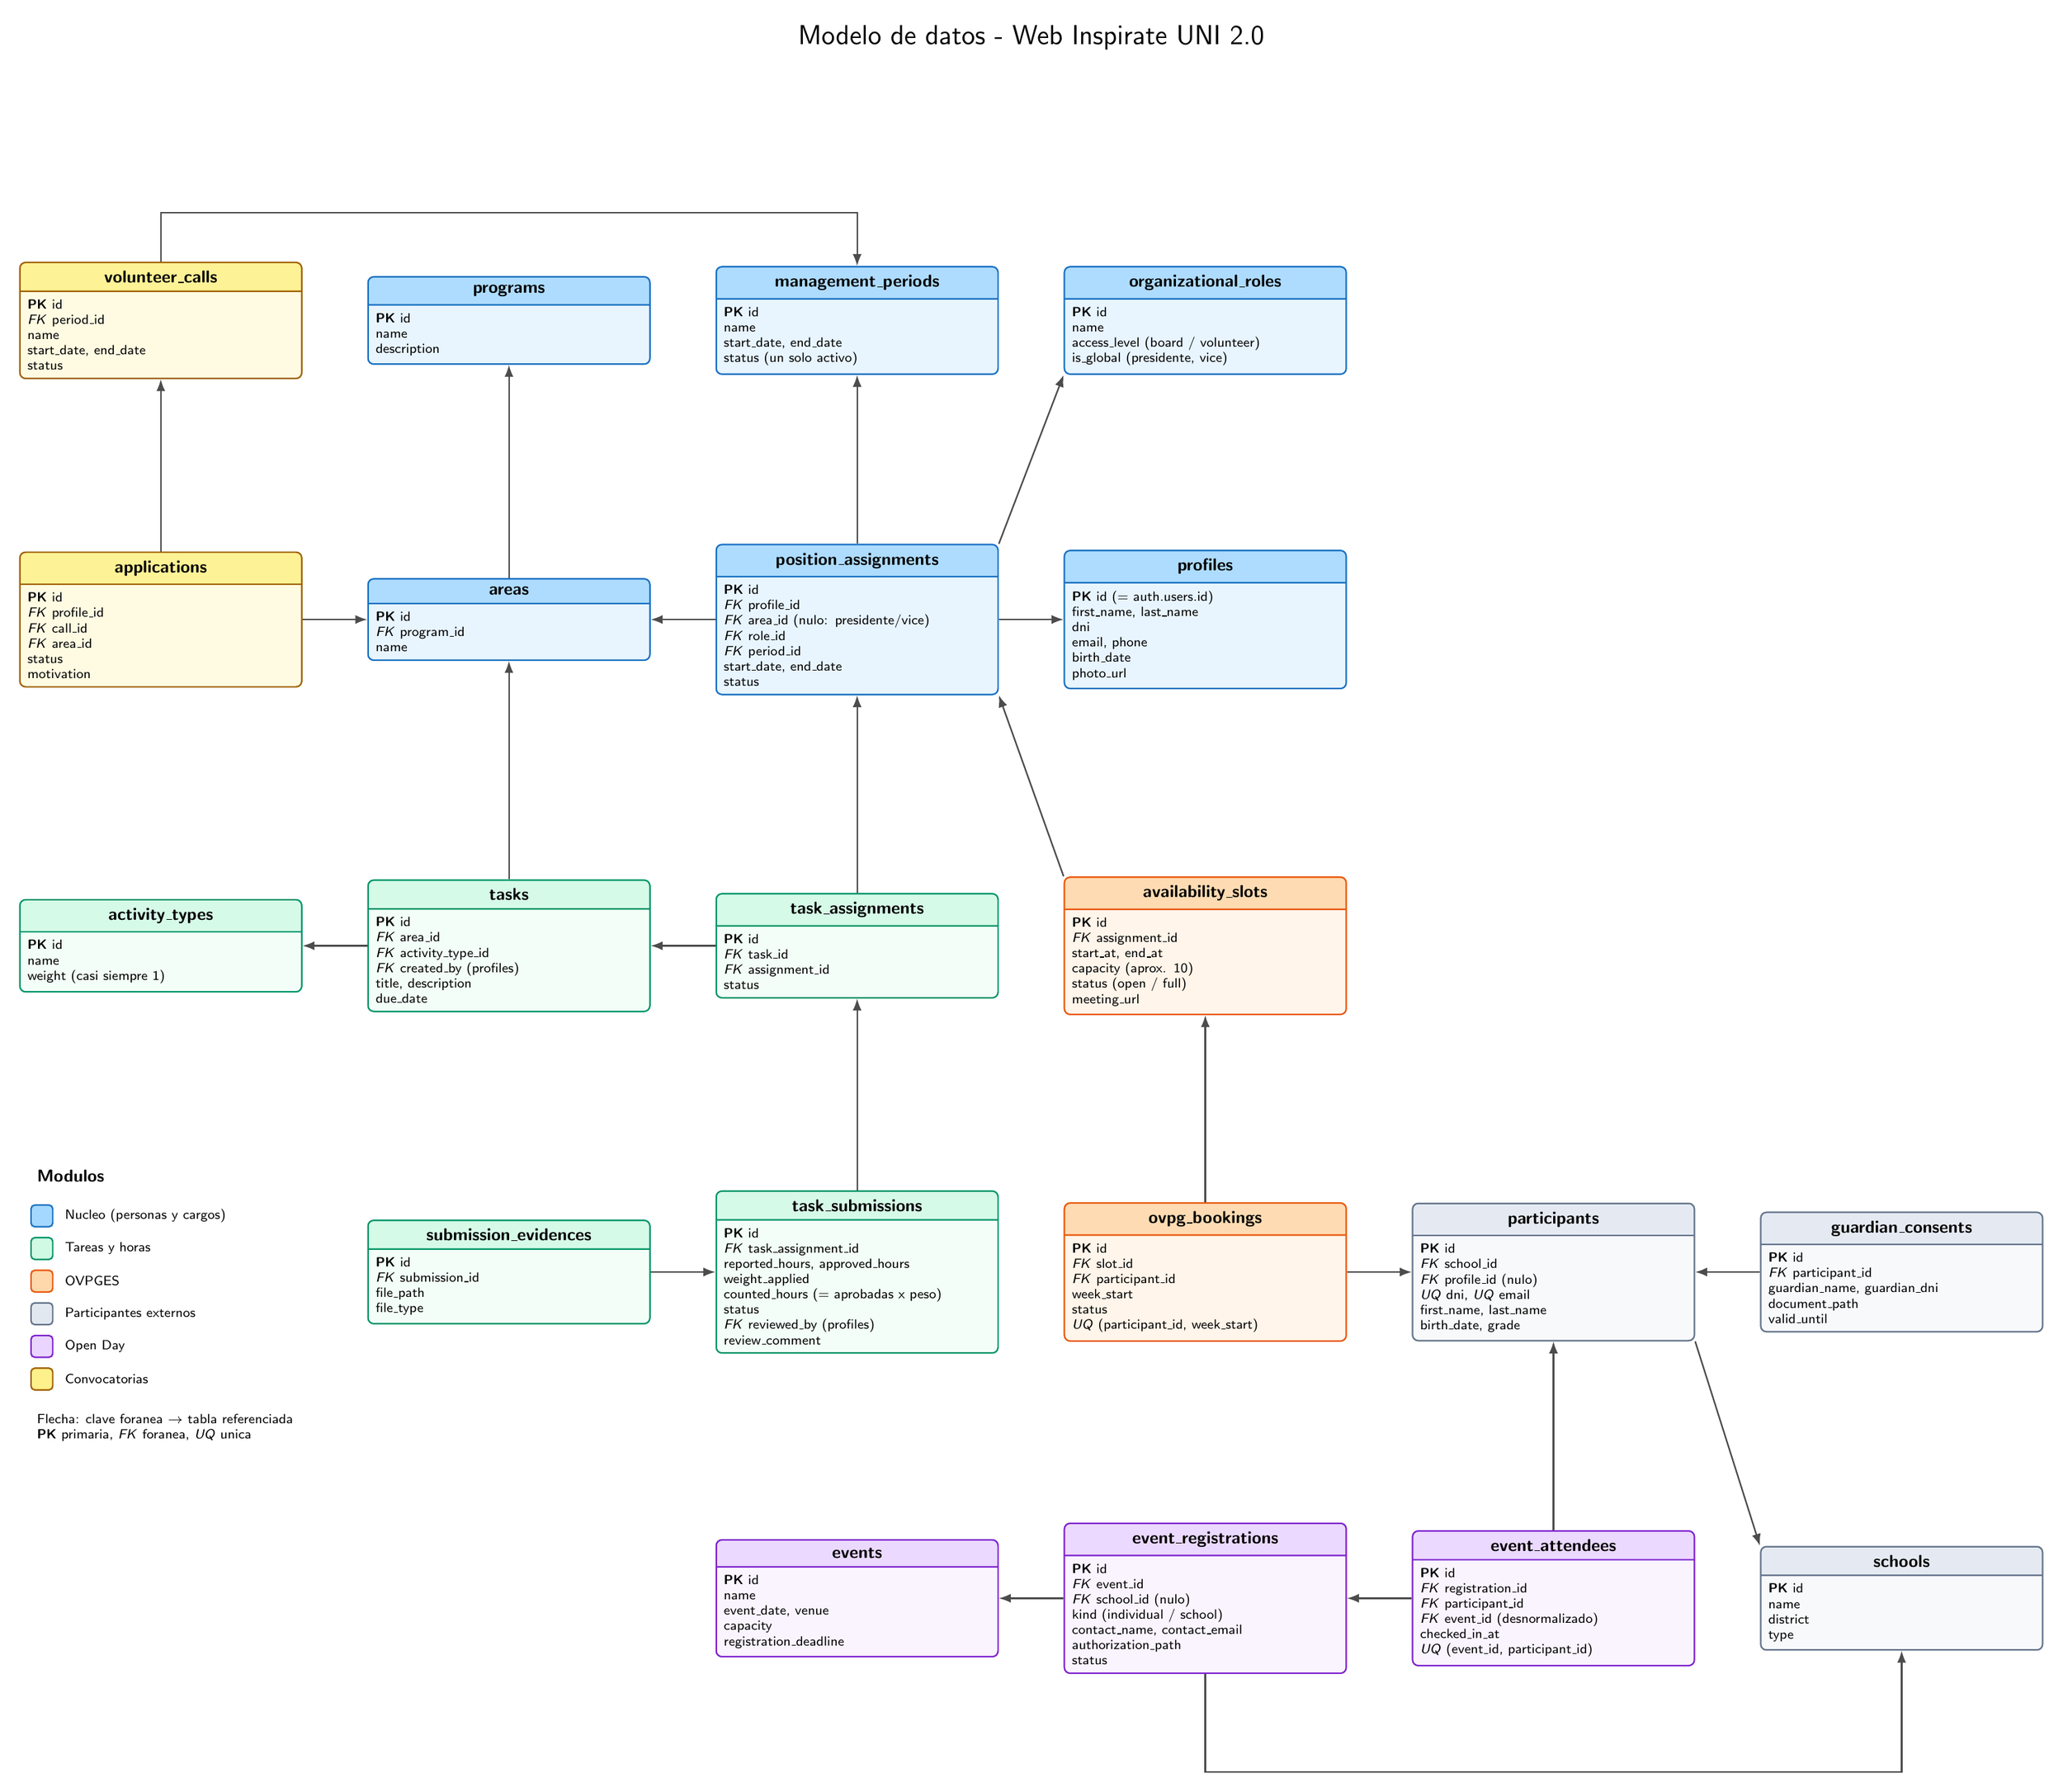
\begin{tikzpicture}

    % Titulo
    \node[font=\Large] at (9.6, 5.2) {Modelo de datos - Web Inspirate UNI 2.0};

    % ==========================================
    % Fila 0
    % ==========================================
    \entity{calls}{-6.4}{0}{yellow}{volunteer_calls}{%
        \pk{id}\\ \fk{period_id}\\ name\\ start_date, end_date\\ status}
    \entity{programs}{0}{0}{blue}{programs}{%
        \pk{id}\\ name\\ description}
    \entity{periods}{6.4}{0}{blue}{management_periods}{%
        \pk{id}\\ name\\ start_date, end_date\\ status (un solo activo)}
    \entity{roles}{12.8}{0}{blue}{organizational_roles}{%
        \pk{id}\\ name\\ access_level (board / volunteer)\\ is_global (presidente, vice)}

    % ==========================================
    % Fila 1
    % ==========================================
    \entity{apps}{-6.4}{-5.5}{yellow}{applications}{%
        \pk{id}\\ \fk{profile_id}\\ \fk{call_id}\\ \fk{area_id}\\ status\\ motivation}
    \entity{areas}{0}{-5.5}{blue}{areas}{%
        \pk{id}\\ \fk{program_id}\\ name}
    \entity{pa}{6.4}{-5.5}{blue}{position\_assignments}{%
        \pk{id}\\ \fk{profile_id}\\ \fk{area_id} (nulo: presidente/vice)\\ \fk{role_id}\\ \fk{period_id}\\ start_date, end_date\\ status}
    \entity{profiles}{12.8}{-5.5}{blue}{profiles}{%
        \pk{id} (= auth.users.id)\\ first_name, last_name\\ dni\\ email, phone\\ birth_date\\ photo_url}

    % ==========================================
    % Fila 2
    % ==========================================
    \entity{atypes}{-6.4}{-11.5}{green}{activity\_types}{%
        \pk{id}\\ name\\ weight (casi siempre 1)}
    \entity{tasks}{0}{-11.5}{green}{tasks}{%
        \pk{id}\\ \fk{area_id}\\ \fk{activity_type_id}\\ \fk{created_by} (profiles)\\ title, description\\ due_date}
    \entity{ta}{6.4}{-11.5}{green}{task\_assignments}{%
        \pk{id}\\ \fk{task_id}\\ \fk{assignment_id}\\ status}
    \entity{slots}{12.8}{-11.5}{orange}{availability\_slots}{%
        \pk{id}\\ \fk{assignment_id}\\ start_at, end_at\\ capacity (aprox. 10)\\ status (open / full)\\ meeting_url}

    % ==========================================
    % Fila 3
    % ==========================================
    \entity{evid}{0}{-17.5}{green}{submission\_evidences}{%
        \pk{id}\\ \fk{submission_id}\\ file_path\\ file_type}
    \entity{subs}{6.4}{-17.5}{green}{task\_submissions}{%
        \pk{id}\\ \fk{task_assignment_id}\\ reported_hours, approved_hours\\ weight_applied\\ counted_hours (= aprobadas x peso)\\ status\\ \fk{reviewed_by} (profiles)\\ review_comment}
    \entity{book}{12.8}{-17.5}{orange}{ovpg\_bookings}{%
        \pk{id}\\ \fk{slot_id}\\ \fk{participant_id}\\ week_start\\ status\\ \uq{(participant_id, week_start)}}
    \entity{part}{19.2}{-17.5}{gray}{participants}{%
        \pk{id}\\ \fk{school_id}\\ \fk{profile_id} (nulo)\\ \uq{dni}, \uq{email}\\ first_name, last_name\\ birth_date, grade}
    \entity{guard}{25.6}{-17.5}{gray}{guardian\_consents}{%
        \pk{id}\\ \fk{participant_id}\\ guardian_name, guardian_dni\\ document_path\\ valid_until}

    % ==========================================
    % Fila 4
    % ==========================================
    \entity{events}{6.4}{-23.5}{purple}{events}{%
        \pk{id}\\ name\\ event_date, venue\\ capacity\\ registration_deadline}
    \entity{reg}{12.8}{-23.5}{purple}{event\_registrations}{%
        \pk{id}\\ \fk{event_id}\\ \fk{school_id} (nulo)\\ kind (individual / school)\\ contact_name, contact_email\\ authorization_path\\ status}
    \entity{att}{19.2}{-23.5}{purple}{event\_attendees}{%
        \pk{id}\\ \fk{registration_id}\\ \fk{participant_id}\\ \fk{event_id} (desnormalizado)\\ checked_in_at\\ \uq{(event_id, participant_id)}}
    \entity{schools}{25.6}{-23.5}{gray}{schools}{%
        \pk{id}\\ name\\ district\\ type}

    % ==========================================
    % Relaciones (FK -> PK)
    % ==========================================
    % Nucleo
    \draw[fkline] (areas) -- (programs);
    \draw[fkline] (pa) -- (areas);
    \draw[fkline] (pa) -- (periods);
    \draw[fkline] (pa) -- (profiles);
    \draw[fkline] (pa.north east) -- (roles.south west);

    % Convocatorias
    \draw[fkline] (calls.north) -- ++(0,0.9) -| (periods.north);
    \draw[fkline] (apps) -- (calls);
    \draw[fkline] (apps) -- (areas);

    % Tareas y horas
    \draw[fkline] (tasks) -- (areas);
    \draw[fkline] (tasks) -- (atypes);
    \draw[fkline] (ta) -- (tasks);
    \draw[fkline] (ta) -- (pa);
    \draw[fkline] (subs) -- (ta);
    \draw[fkline] (evid) -- (subs);

    % OVPGES
    \draw[fkline] (slots.north west) -- (pa.south east);
    \draw[fkline] (book) -- (slots);
    \draw[fkline] (book) -- (part);

    % Participantes
    \draw[fkline] (guard) -- (part);
    \draw[fkline] (part.south east) -- (schools.north west);

    % Open Day
    \draw[fkline] (reg) -- (events);
    \draw[fkline] (att) -- (reg);
    \draw[fkline] (att) -- (part);
    \draw[fkline] (reg.south) -- ++(0,-1.8) -| (schools.south);

    % ==========================================
    % Leyenda
    % ==========================================
    \node[anchor=north west, font=\scriptsize] (lg) at (-8.8, -15.5) {\textbf{\small Modulos}};
    \node[mod, fill=boxblue, draw=borderblue, anchor=west] (l1) at ($(lg.south west)+(0,-0.5)$) {};
    \node[font=\scriptsize, anchor=west] at (l1.east) {\ Nucleo (personas y cargos)};
    \node[mod, fill=boxgreen, draw=bordergreen, anchor=west] (l2) at ($(l1.west)+(0,-0.6)$) {};
    \node[font=\scriptsize, anchor=west] at (l2.east) {\ Tareas y horas};
    \node[mod, fill=boxorange, draw=borderorange, anchor=west] (l3) at ($(l2.west)+(0,-0.6)$) {};
    \node[font=\scriptsize, anchor=west] at (l3.east) {\ OVPGES};
    \node[mod, fill=boxgray, draw=bordergray, anchor=west] (l4) at ($(l3.west)+(0,-0.6)$) {};
    \node[font=\scriptsize, anchor=west] at (l4.east) {\ Participantes externos};
    \node[mod, fill=boxpurple, draw=borderpurple, anchor=west] (l5) at ($(l4.west)+(0,-0.6)$) {};
    \node[font=\scriptsize, anchor=west] at (l5.east) {\ Open Day};
    \node[mod, fill=boxyellow, draw=borderyellow, anchor=west] (l6) at ($(l5.west)+(0,-0.6)$) {};
    \node[font=\scriptsize, anchor=west] at (l6.east) {\ Convocatorias};
    \node[font=\scriptsize, anchor=west, align=left] at ($(l6.west)+(0,-0.9)$)
        {Flecha: clave foranea $\rightarrow$ tabla referenciada\\ \textbf{PK} primaria, \textit{FK} foranea, \textit{UQ} unica};

\end{tikzpicture}
\end{document}
